\section{反馈控制问题的类别}\label{5Aref}
考虑下述系统
\begin{equation}
    \begin{aligned}
  \dot{x} = f (t, x, u)\\
  y = h (t, x, u)
\end{aligned}\label{sys:1}
\end{equation}

\textbf{1. 状态反馈镇定问题:}目标是设计一反馈控制律
\[ u = \gamma (t, x) \]
使得$x = 0$是下述闭环系统的一致渐近稳定的平衡点
\[ \dot{x} = f (t, x, \gamma (t, x)) \]
可分为:
\begin{itemize}[leftmargin=1em]
    \item 静态状态反馈:$u = \gamma (t, x)$
    \item 动态状态反馈:$u = \gamma (t, x, z), \dot{z} = g (t, x, z)$。上一章中的自适应控制即属此类。
\end{itemize}

\textbf{2. 输出反馈镇定问题:}
可分为:
\begin{itemize}[leftmargin=1em]
\item 静态输出反馈:$u = \gamma (t, y)$
\item 动态输出反馈:$u = \gamma (t, y, z), \dot{z} = g (t, y, z)$。状态观测器即属此类。
\end{itemize}

\begin{example}
  考虑如下线性定常系统
  \[ \dot{x} = A x + B u \]
 \begin{itemize}[leftmargin=1em]
  \item 状态反馈:$u = - K x$,从而$\dot{x} = A x + B u = (A - B K) x$,目标是使$A - B K$是Hurwitz的;
  
  \item 输出反馈:设$y=Cx+Du$。

  \begin{center}
      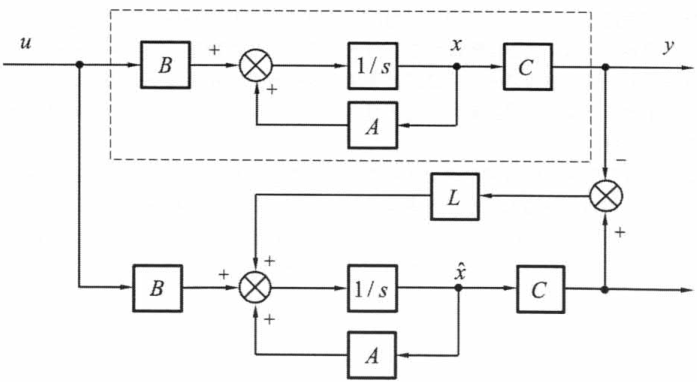
\includegraphics[width=0.5\linewidth]{figure/adaptive/state_observer.png}
      \captionof{figure}{全维状态观测器的结构}
      \label{fig:state-observer}
  \end{center}
  
  定义观测得的状态为$\hat{x}$,观测器输出$\hat{y} = C  \hat{x} + D  u$,则如上图,
  $\dot{\hat{x}} = A  \hat{x} + B  u + L(y - \hat{y})$。

  定义$u =\gamma(t,y,\hat{x})= - K \hat{x}$。则$\dot{x} = A x - B K \hat{x}=Ax-BK(x-e)=(A-BK)x+BKe$——目标之一:$A-BK$是Hurwitz的;
  
  又定义$e = x - \hat{x}$,则$\dot{e} = A e - L C e = (A - L C) e$,——目标之二:$A - L C$是Hurwitz的。  
  \end{itemize}
\end{example}

\textbf{3. 跟踪问题:}
\begin{itemize}[leftmargin=1em]
    \item 状态跟踪:$x \rightarrow x_d (t)$,目的是使$e = x - x_d$趋于$0$;
    \item 输出跟踪:$y \rightarrow y_d (t)$,目的是使$e = y - y_d$趋于$0$。
\end{itemize}